%!TEX root = ../Thesis.tex
\section{Tests}\label{Tests}
\subsection{Automatische Tests}
Für die relevantesten Funktionen der Anwendung wurden Unit-Tests geschrieben.
Im Backend sowie Frontend wurden die Frameworks Chai\footnote{\cite{chai}} und Mocha\footnote{\cite{mocha}} verwendet.
Chai ist eine Assertion Library, während Mocha ein komplettes Test-Framework ist.
Die Struktur der Tests wird somit durch Mocha vorgebenen.
Durch Chai werden lediglich die Assertions evaluiert.
\\
Die Testklassen heißen jeweils testMain.js und befinden sich in den src/test Ordnern des Front- und Backends.
\\
\subsubsection*{Testabdeckung}
Die erreichte Testabdeckungen ist in \autoref{fig:tc_frontend} und \autoref{fig:tc_backend} zu sehen.
\begin{figure}[H]
    \centering
    \begin{minipage}[t]{1\textwidth}
        \caption{Testabdeckung Frontend}
        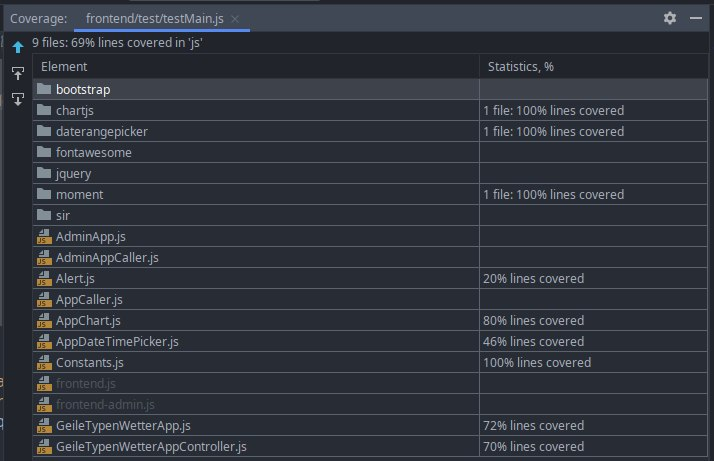
\includegraphics[width=1\textwidth]{img/tc_frontend2.png}\\
        \source{Eigene Darstellung}
        \label{fig:tc_frontend}
    \end{minipage}
\end{figure}
\begin{figure}[H]
    \centering
    \begin{minipage}[t]{1\textwidth}
        \caption{Testabdeckung Backend}
        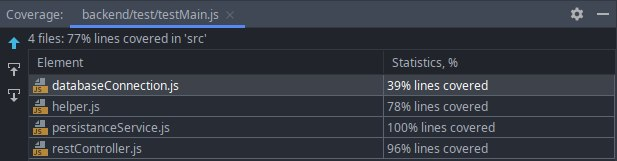
\includegraphics[width=1\textwidth]{img/tc_backend2.png}\\
        \source{Eigene Darstellung}
        \label{fig:tc_backend}
    \end{minipage}
\end{figure}
\subsection{Manuelle Klicktests}
Es wurden manuelle Tests der Benutzoberfläche ausgeführt, um etwaige Fehler dort zu entdecken.
Diese wurden dokumentiert.
\subsubsection*{Inhalte}
Es sollen folgende Inhalte dokumentiert werden:
\begin{itemize}
    \item Git Commit Hash (Programmversion)
    \item Git Branch
    \item Verwendetes Betriebssystem
    \item Verwendeter Browser inkl. Build
    \item Screenshots bei Darstellungsfehlern
    \item Bildschirmauflösung, insbesonders bei mobiler Ansicht
\end{itemize}
Darüber hinaus wurde die Anwendung in der mobilen (responsiven) Ansicht getestet, was ebenfalls dokumentiert wurde.
Die Testdurchführung befindet sich in \autoref{anh:testplan}.

